% Original vector reconstruction of source Fig.81.3, PDF332 / printed320.
% These are the two Fig.81.2 color graphs. Arrows now carry color.
% Three paths in either panel:
%   quark1 -> gluon4 upper strand;
%   gluon4 lower strand -> gluon3 upper strand;
%   gluon3 lower strand -> quark2.
% Reading against the arrows from leg2 gives (T^{a3}T^{a4})_{i2}^{i1}.
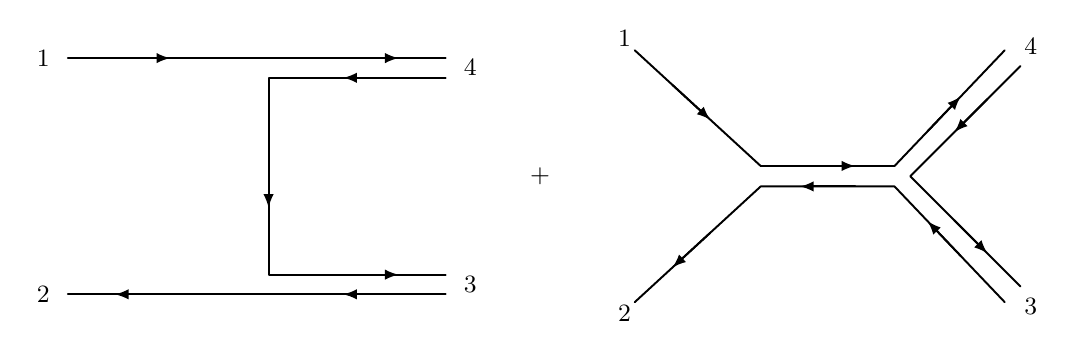
\begin{tikzpicture}[x=1mm,y=1mm,line width=.7pt,>=latex,
  line cap=round,line join=round,font=\fontsize{9.5}{11.5}\selectfont]
  \begin{scope}[shift={(29,0)}]
    \draw (-24,15)--(24,15);
    \draw (24,12.5)--(1.5,12.5)--(1.5,-12.5)--(24,-12.5);
    \draw (24,-15)--(-24,-15);
    \draw[->] (-18,15)--(-11,15);
    \draw[->] (11,15)--(18,15);
    \draw[->] (18,12.5)--(11,12.5);
    \draw[->] (1.5,4)--(1.5,-4);
    \draw[->] (11,-12.5)--(18,-12.5);
    \draw[->] (18,-15)--(11,-15);
    \draw[->] (-11,-15)--(-18,-15);
    \node[left] at (-25,15) {$1$};
    \node[left] at (-25,-15) {$2$};
    \node[right] at (25,-13.75) {$3$};
    \node[right] at (25,13.75) {$4$};
  \end{scope}
  \node at (65,0) {$+$};
  \begin{scope}[shift={(101,0)}]
    \draw (-24,16)--(-8,1.3)--(9,1.3)--(23,16);
    \draw (25,14)--(11,0)--(25,-14);
    \draw (23,-16)--(9,-1.3)--(-8,-1.3)--(-24,-16);
    \draw[->] (-19.2,11.59)--(-14.4,7.18);
    \draw[->] (-3,1.3)--(4,1.3);
    \draw[->] (13.2,5.71)--(17.4,10.12);
    \draw[->] (20.8,9.8)--(16.6,5.6);
    \draw[->] (16.6,-5.6)--(20.8,-9.8);
    \draw[->] (17.4,-10.12)--(13.2,-5.71);
    \draw[->] (4,-1.3)--(-3,-1.3);
    \draw[->] (-14.4,-7.18)--(-19.2,-11.59);
    \node[above left,inner sep=1pt] at (-24,16) {$1$};
    \node[below left,inner sep=1pt] at (-24,-16) {$2$};
    \node[below right,inner sep=1pt] at (25,-15) {$3$};
    \node[above right,inner sep=1pt] at (25,15) {$4$};
  \end{scope}
\end{tikzpicture}

